\subsection{Virtual Rapport 2.0}
\label{sub:sec:virtualrapport2}

Huang et. al. developed a short-term rapport virtual agent to enhance mutual attention and coordination using backchannels through a data-driven approach that takes into account context-specific response models in a dyadic conversational setting~\cite{Buschmeier2011}. The model determines the best suitable timings to generate specific backchannel behaviours and turn-taking opportunities according to the perceptual state observed.

%%%%%%%%%%%%%%%%%%%%%%%%%%%%%%%%%%%%%%%%%%%%%%%%%%%%%%%%%%%%%%%%%%%%%%%%%%%%%%%%%%%%%

\subsubsection*{System description}

Following Figure~\ref{fig:virtualrapport2System}, the system contains the following modules:
\begin{itemize}
	\item \textbf{\textit{Perception}}: analyses human speaker's behaviour in real time;
	\item \textbf{\textit{Response Models}}: predicts timing of backchannel feedback and end-of-turn opportunities in real time using information from the environment and from the agent itself. It also decides which behaviour to generate;
	\item \textbf{\textit{Consensus Data}}: contains data collected from Rapport 06-07\footnote{\url{http://rapport.ict.usc.edu}} dataset and self-disclosure data-set using \ac{PCS}. The data contains dyadic interactions between a human speaker telling a story and human silent listener;
	\item \textbf{\textit{Generation}}: generates the output from the response models.
\end{itemize}

\begin{figure}[hbt]
  \centering
  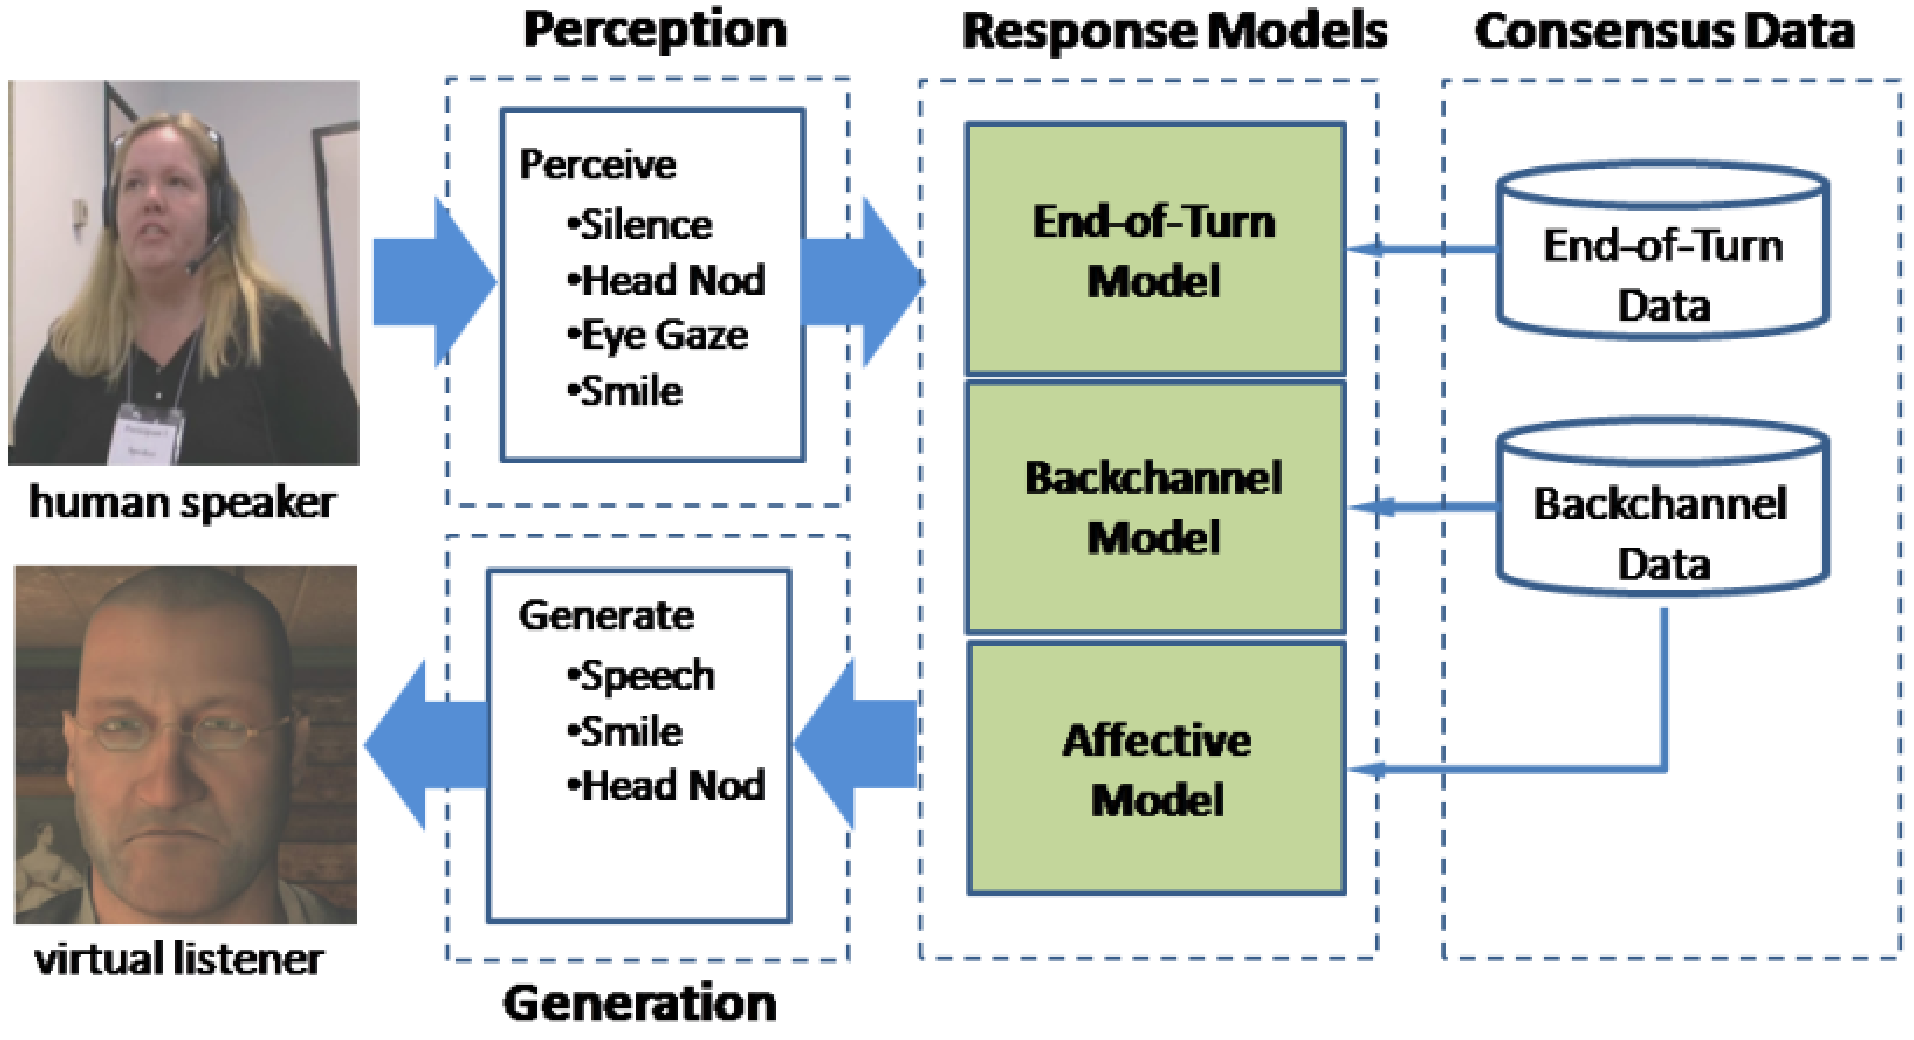
\includegraphics[width=0.65\textwidth]{Images/VirtualRapport2_System.png}
  \caption{Architecture of Virtual Rapport 2.0. From~\cite{Buschmeier2011}.}
  \label{fig:virtualrapport2System}
\end{figure} 

As depicted in Figure \ref{fig:virtualrapport2System} there are three models in the \textit{Response Models} module: \textit{End-of-turn}, \textit{Backchannel}, and \textit{Affective} that are described below.

The first model, \textit{end-of-turn}, using a rule-based approach, identifies turn-taking opportunities by analysing the current speaker's non-verbal behaviours. For example, if the human interrupts the virtual agent, the agent stops, yields his turn and, says ``I am sorry, keep going'' while showing a facial expression~\cite{Buschmeier2011}, showing, at the same time, signs of friendliness (enhancing positivity).

The second model, \textit{Backchannel}, is \ac{ML}-based (using forward-only inference \ac{CRF}~\cite{Bishop2006} for real-time predictions) and trained using the Rapport 06-07 dataset. It is capable of predicting when and how to give non-verbal feedback.

The last model, \textit{Affective}, analyses facial feature points in real time and detects whenever the speaker is smiling.
 
During the interaction, the three response models are used in conjunction to decide whenever it is appropriate to generate a backchannel. If the speaker is smiling (according to the \textit{Affective} model) and if it is a good opportunity to generate a backchannel (according to the \textit{Backchannel} model) then a head nod (one of the three identified in their studies) is generated accompanied by a smile.

%%%%%%%%%%%%%%%%%%%%%%%%%%%%%%%%%%%%%%%%%%%%%%%%%%%%%%%%%%%%%%%%%%%%%%%%%%%%%%%%%%%%%%%%
\subsubsection*{Evaluation}
The developed virtual agent interacted with the human subjects in an interview environment in which the former was the interviewer and the later the interviewed. With the goal of comparing the developed system with the previous version~\cite{Gratch2006}, the evaluation measured the following dimensions: five-item social presence scale~\cite{Bailenson2001}, overall naturalness, backchannel feedback and end-of-turn prediction.


%%%%%%%%%%%%%%%%%%%%%%%%%%%%%%%%%%%%%%%%%%%%%%%%%%%%%%%%%%%%%%%%%%%%%%%%%%%%%%%%%%%%%%%%

\subsubsection*{Discussion}
The results demonstrate a significant improvement over the previous version. Over 90\% of the users preferred the Virtual Rapport 2.0 rapport agent over the previous rule-based system~\cite{Gratch2006, Morency2008}. The timing's precision and recall were far better, leading to a better synchronism and perceived naturalness from the user during the interaction. According to the authors, the data-driven design, the much richer set of emotions capable of mimicking smiles, and the generation of more natural head gestures are the best indicators explaining the overall better results on the stronger feelings of rapport.

To conclude the most relevant aspects of the system are:
\begin{itemize}
	\item Identification of different head nods patterns;
	\item The duality of \ac{ML}-based decisions and affective model to generate backchannel behaviour;
	\item Elegant strategy for handling interruptions.
\end{itemize}